% Chapter 2
\chapter[Experimental approach of surpressing the spectral diffusion]{Experimental approach of surpressing the spectral diffusion} % Main chapter title

\label{Chapter2} % Change X to a consecutive number; for referencing this chapter elsewhere, use \ref{ChapterX}

%----------------------------------------------------------------------------------------
%	SECTION 1
%----------------------------------------------------------------------------------------

\section[sample preparation]{sample preparation}
\subsection{preparation of the substrate}
\paragraph{IIa diamond as substrate}

Our choice of substrate is based on the principle of low background fluorescence, low refractive index and high thermal conductivity at low temperature (4K) and no misleading spectral features.

\paragraph{here is a paragraph dedicate to the expended explanation of requirements of substrate} 
\paragraph{here is a paragraph describing that based on the mentioned principles, Uwe Jantzen and coworkers has compared several different materials and in the end type IIa diamond rised as the most fitting candidate.}
\paragraph{FIB}
In order to make it more convenient to trace the nanodiamonds, markers were curved onto the surface of the IIa type diamond substrate, this work was done by Uwe Jantzen during his master's thesis period. As is shown in the fig.[], the focues ion beam bombards the surface of diamond away and leaves behind markers that are visible in optical microscopy images and SEM images, as well as confocal microscopy images.
\paragraph{here is a sketch of how Ga-ion bombards the surface of substrate}
\paragraph{here insert image of markers, optical, sem and confocal}
\paragraph{fig. ?.  }



\subsection{spin-coating of the sample}
\subsubsection{theory of spin coating} 
Spin coating is the method that spreads the liquid evenly across the surface of 

thickness $\sim$ $\frac{1}{\sqrt{\omega}}$, time of evaporation, single time or multiple times. Surface condition and liquid spreading. Importance of clean room. Before and after optical image.
%-----------------------------------
\subsubsection{Acid cleaning}
To make sure that the NDs dispension can evenly spread and eventually settled on the substrate, a smooth, cleaned and hydrophilic surface is important.

Tri acid boiling is a very practicle way of substrate cleaning.

\paragraph{here insert a sketch of how we do acid cleaning} 

the strongly acidic and oxidic mixture can remove most of the contaminations, leaving a clean hydrphilic surface covered with carboxyl and hydroxyl groups.

\paragraph {here insert image of before and after cleaning substrate, optical image, confocal image }
Tri Acid boiling blabla. Expectation of the surface. Before after cleaning. Optical image. Confocal image.

\paragraph{fundamental of spin coating} thickness $\sim$ $\frac{1}{\sqrt{\omega}}$, time of evaporation, single time or multiple times. Surface condition and liquid spreading. Importance of clean room. Before and after optical image.
%-----------------------------------
%	SECTION 2
%-----------------------------------
\section[development of a technology to estimate the spectral diffusion]{development of a technology to estimate the spectral diffusion}

\paragraph{Setup} 

In order to resolve the fine structure of ZPL of SiVs, we need to observe the sample at low temperature, thus a cryogenic setup must be applied.
Our setup is a typical confocal micropscopy setup connects with a cryostat, which cools the sample with liquid Helium flow.

\paragraph{here inserts a picture of our flow cryostat, from out and in side.}
This is the flow cryostat, whose main body is a vaccum chamber with

\paragraph{here insert a sketch of the cryo4 setup}
Confocal + Cryostat, Green laser + Red laser, spectrometer, apd, pic


\paragraph{PL} green laser + spectrometer. Instrumental limitation fo resolution from spectrometer. See the sum of all Emission over exposure time. Observing ZPL and phonon side band.

\paragraph{PLE} resonance excitation of optical transition. Rsésolution limited by scanning step of laser. Observing phonon side band with apd. range of scanning: limited by laser, small.

\paragraph{time resolved PL spectra} Tracing PL spectra over time, show the diffusing behaviour of lines, characterisation methods: excitation polarisation: width of diffusion. Cross- correlation over time.
\paragraph{}We recorded and noticed that the diffusion, whose range can up to 1nm, is far beyond the capability of PLE. 

%-----------------------------------
%	SECTION 3
%-----------------------------------
\section{Oxidation}
\paragraph{Effect of Oxidation} Size reducing, surface group changing, removal of Sp2 carbon

\subsection[first Oxidation]{first Oxidation}
\paragraph{method}According to the paper[Elka Neu], condition: . With the help from Markus Mohr. Setup : tube furnace, pic. 

\paragraph{Before Oxidation} Confocal image, SEM image, PL, time resolved PL, PLE. Power dependence.
\begin{figure}[h]
\centering
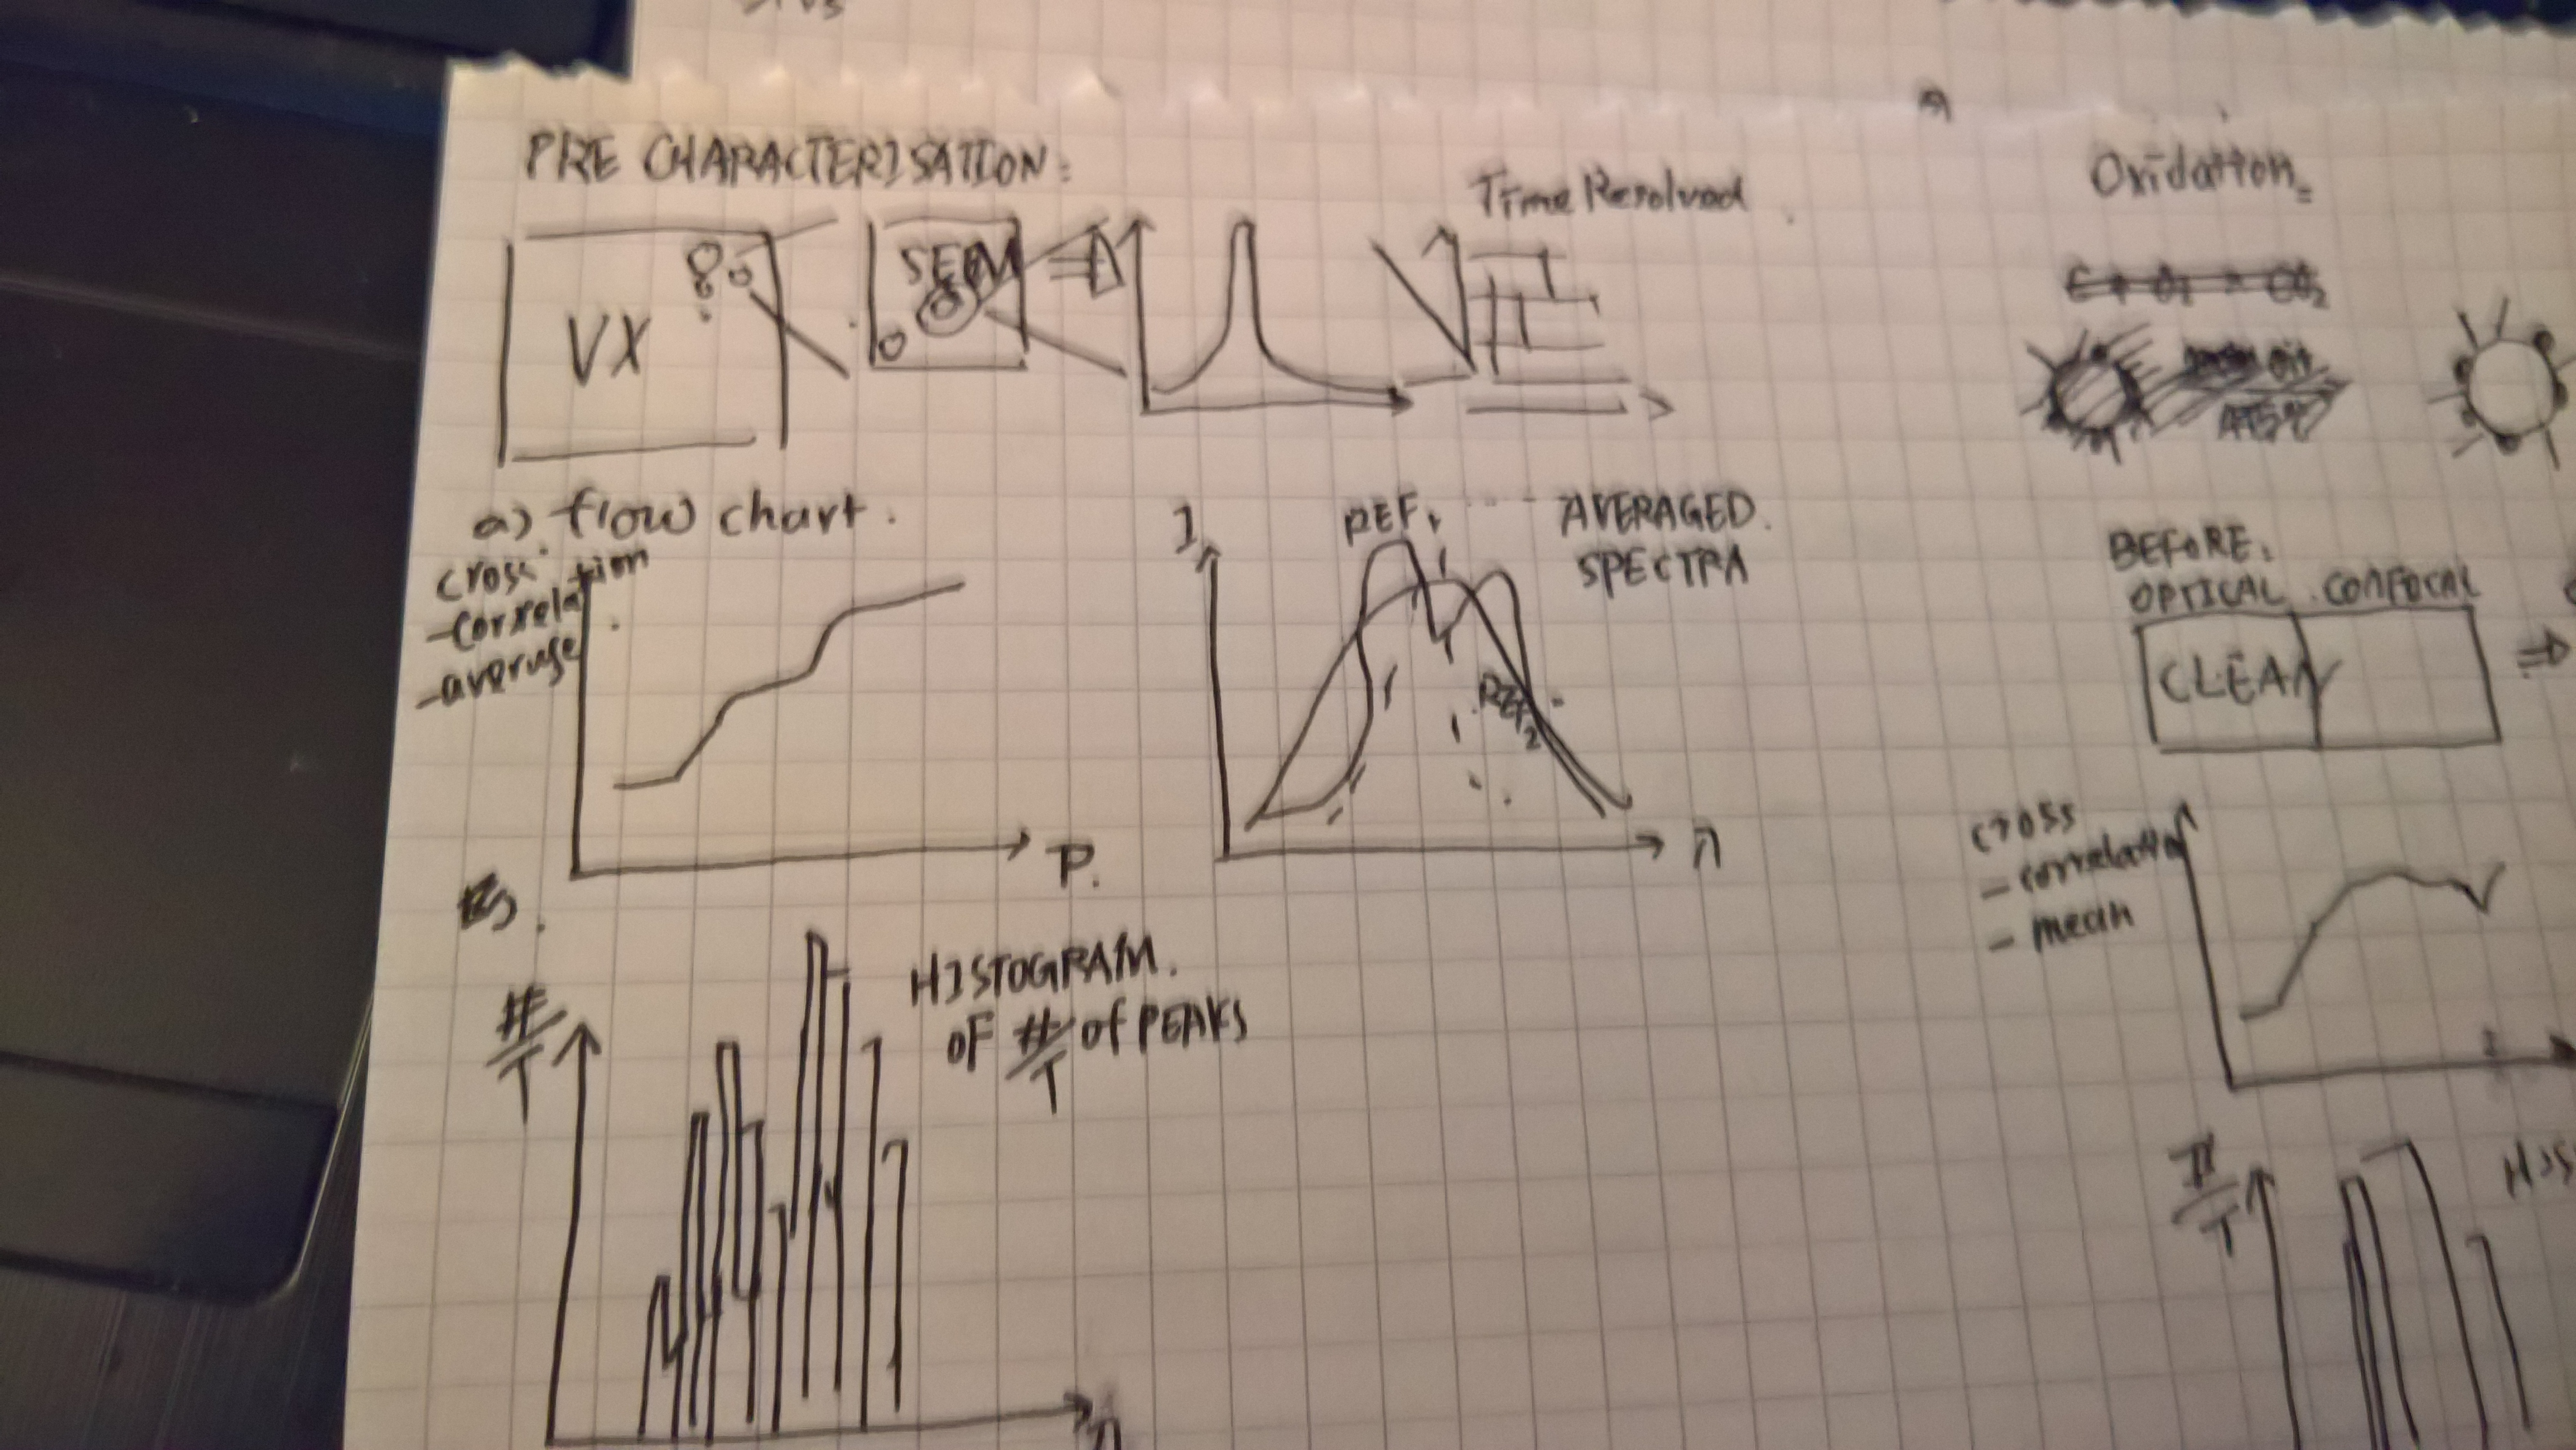
\includegraphics[width=0.7\linewidth]{../pic/WP_20160921_20_41_03_Pro_LI}
\caption{}
\label{fig:wp20160921204103proli}
\end{figure}

\paragraph{After Oxidation}dirty surface: Optical image, Confocal image, time resolved PL. Power dependence.
\begin{figure}[h]
\centering
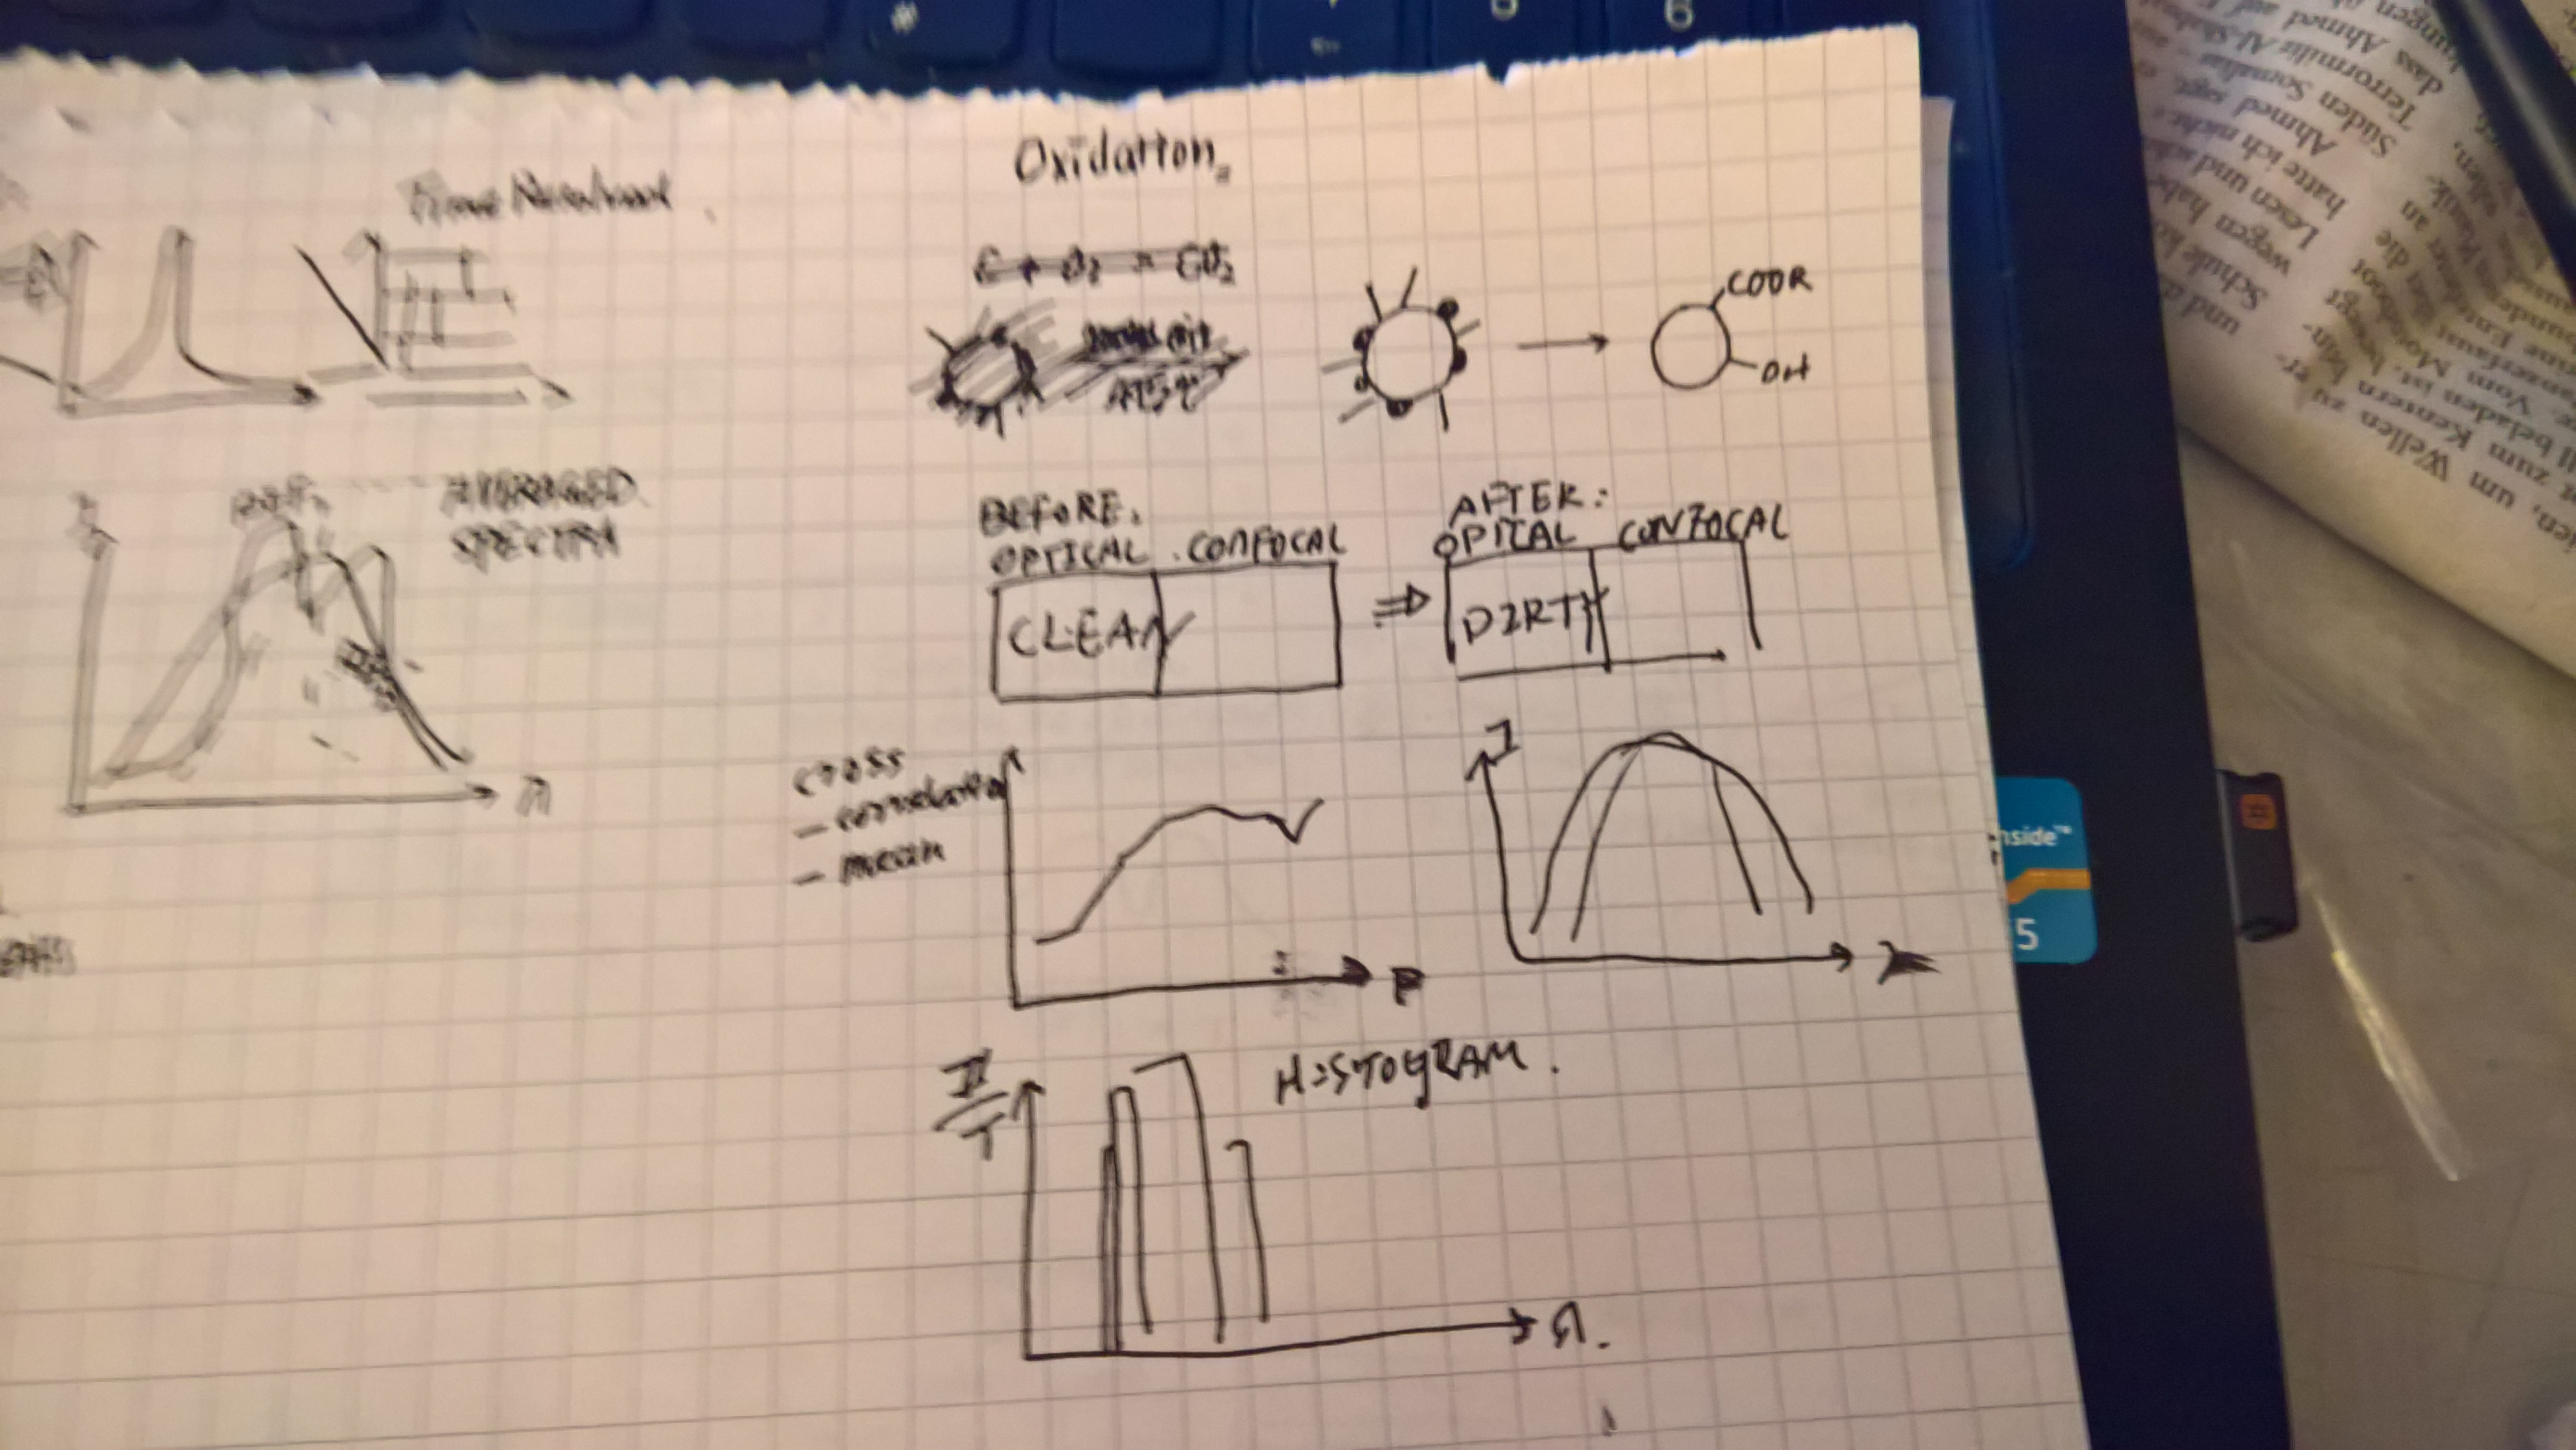
\includegraphics[width=0.7\linewidth]{../pic/WP_20160921_20_41_09_Pro_LI}
\caption{}
\label{fig:wp20160921204109proli}
\end{figure}

\paragraph{Analysis} Reason for getting dirty surface. Behaviour of the lines: brighter, broader...

\subsection[Second Oxidation]{second Oxidation}

\paragraph{method} According to [] paper, higher temperature - total removal of Sp2 carbon. Improvement of setup: to prevent contamination: cleaner tube, clean He flow when cooling. Improvement of characterisation: added in excitation polarisation, record the time resolved PL with 2 differently polarised incident beam. Samller nanodiamonds: a earlier batch.
\begin{figure}[h]
\centering
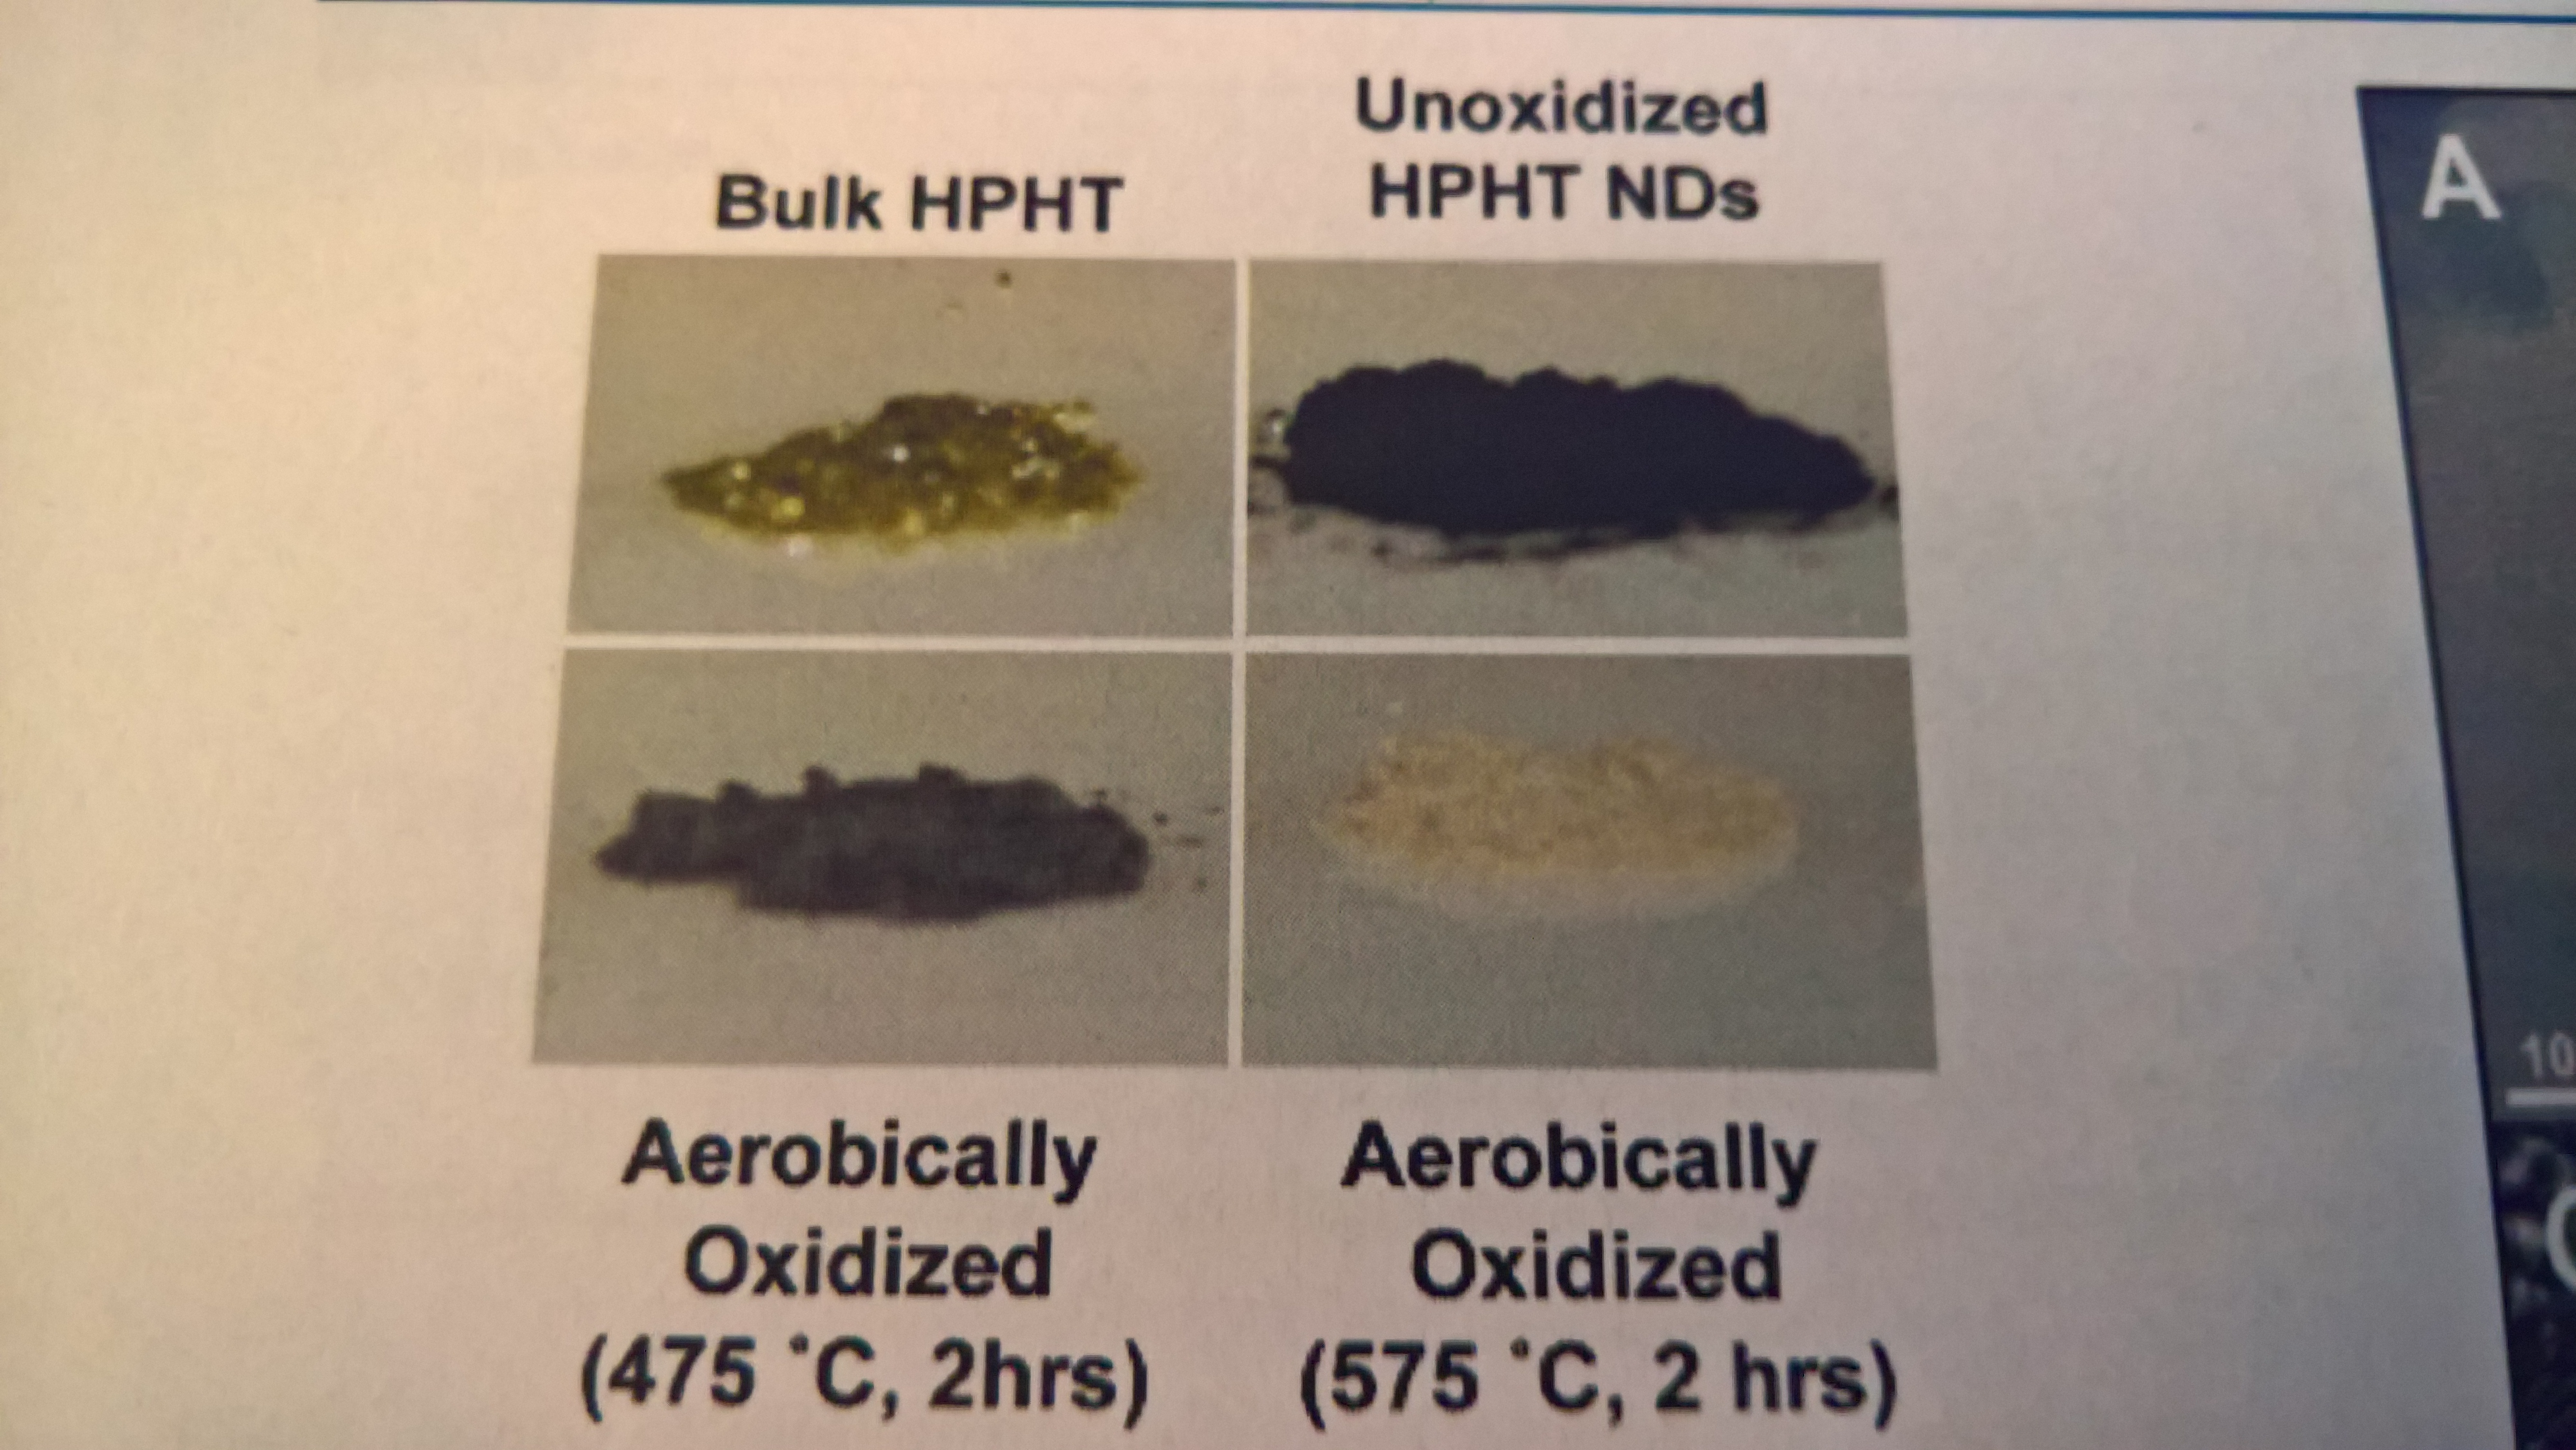
\includegraphics[width=0.7\linewidth]{../pic/WP_20160921_20_43_19_Pro_LI}
\caption{}
\label{fig:wp20160921204319proli}
\end{figure}
\begin{figure}[h]
\centering
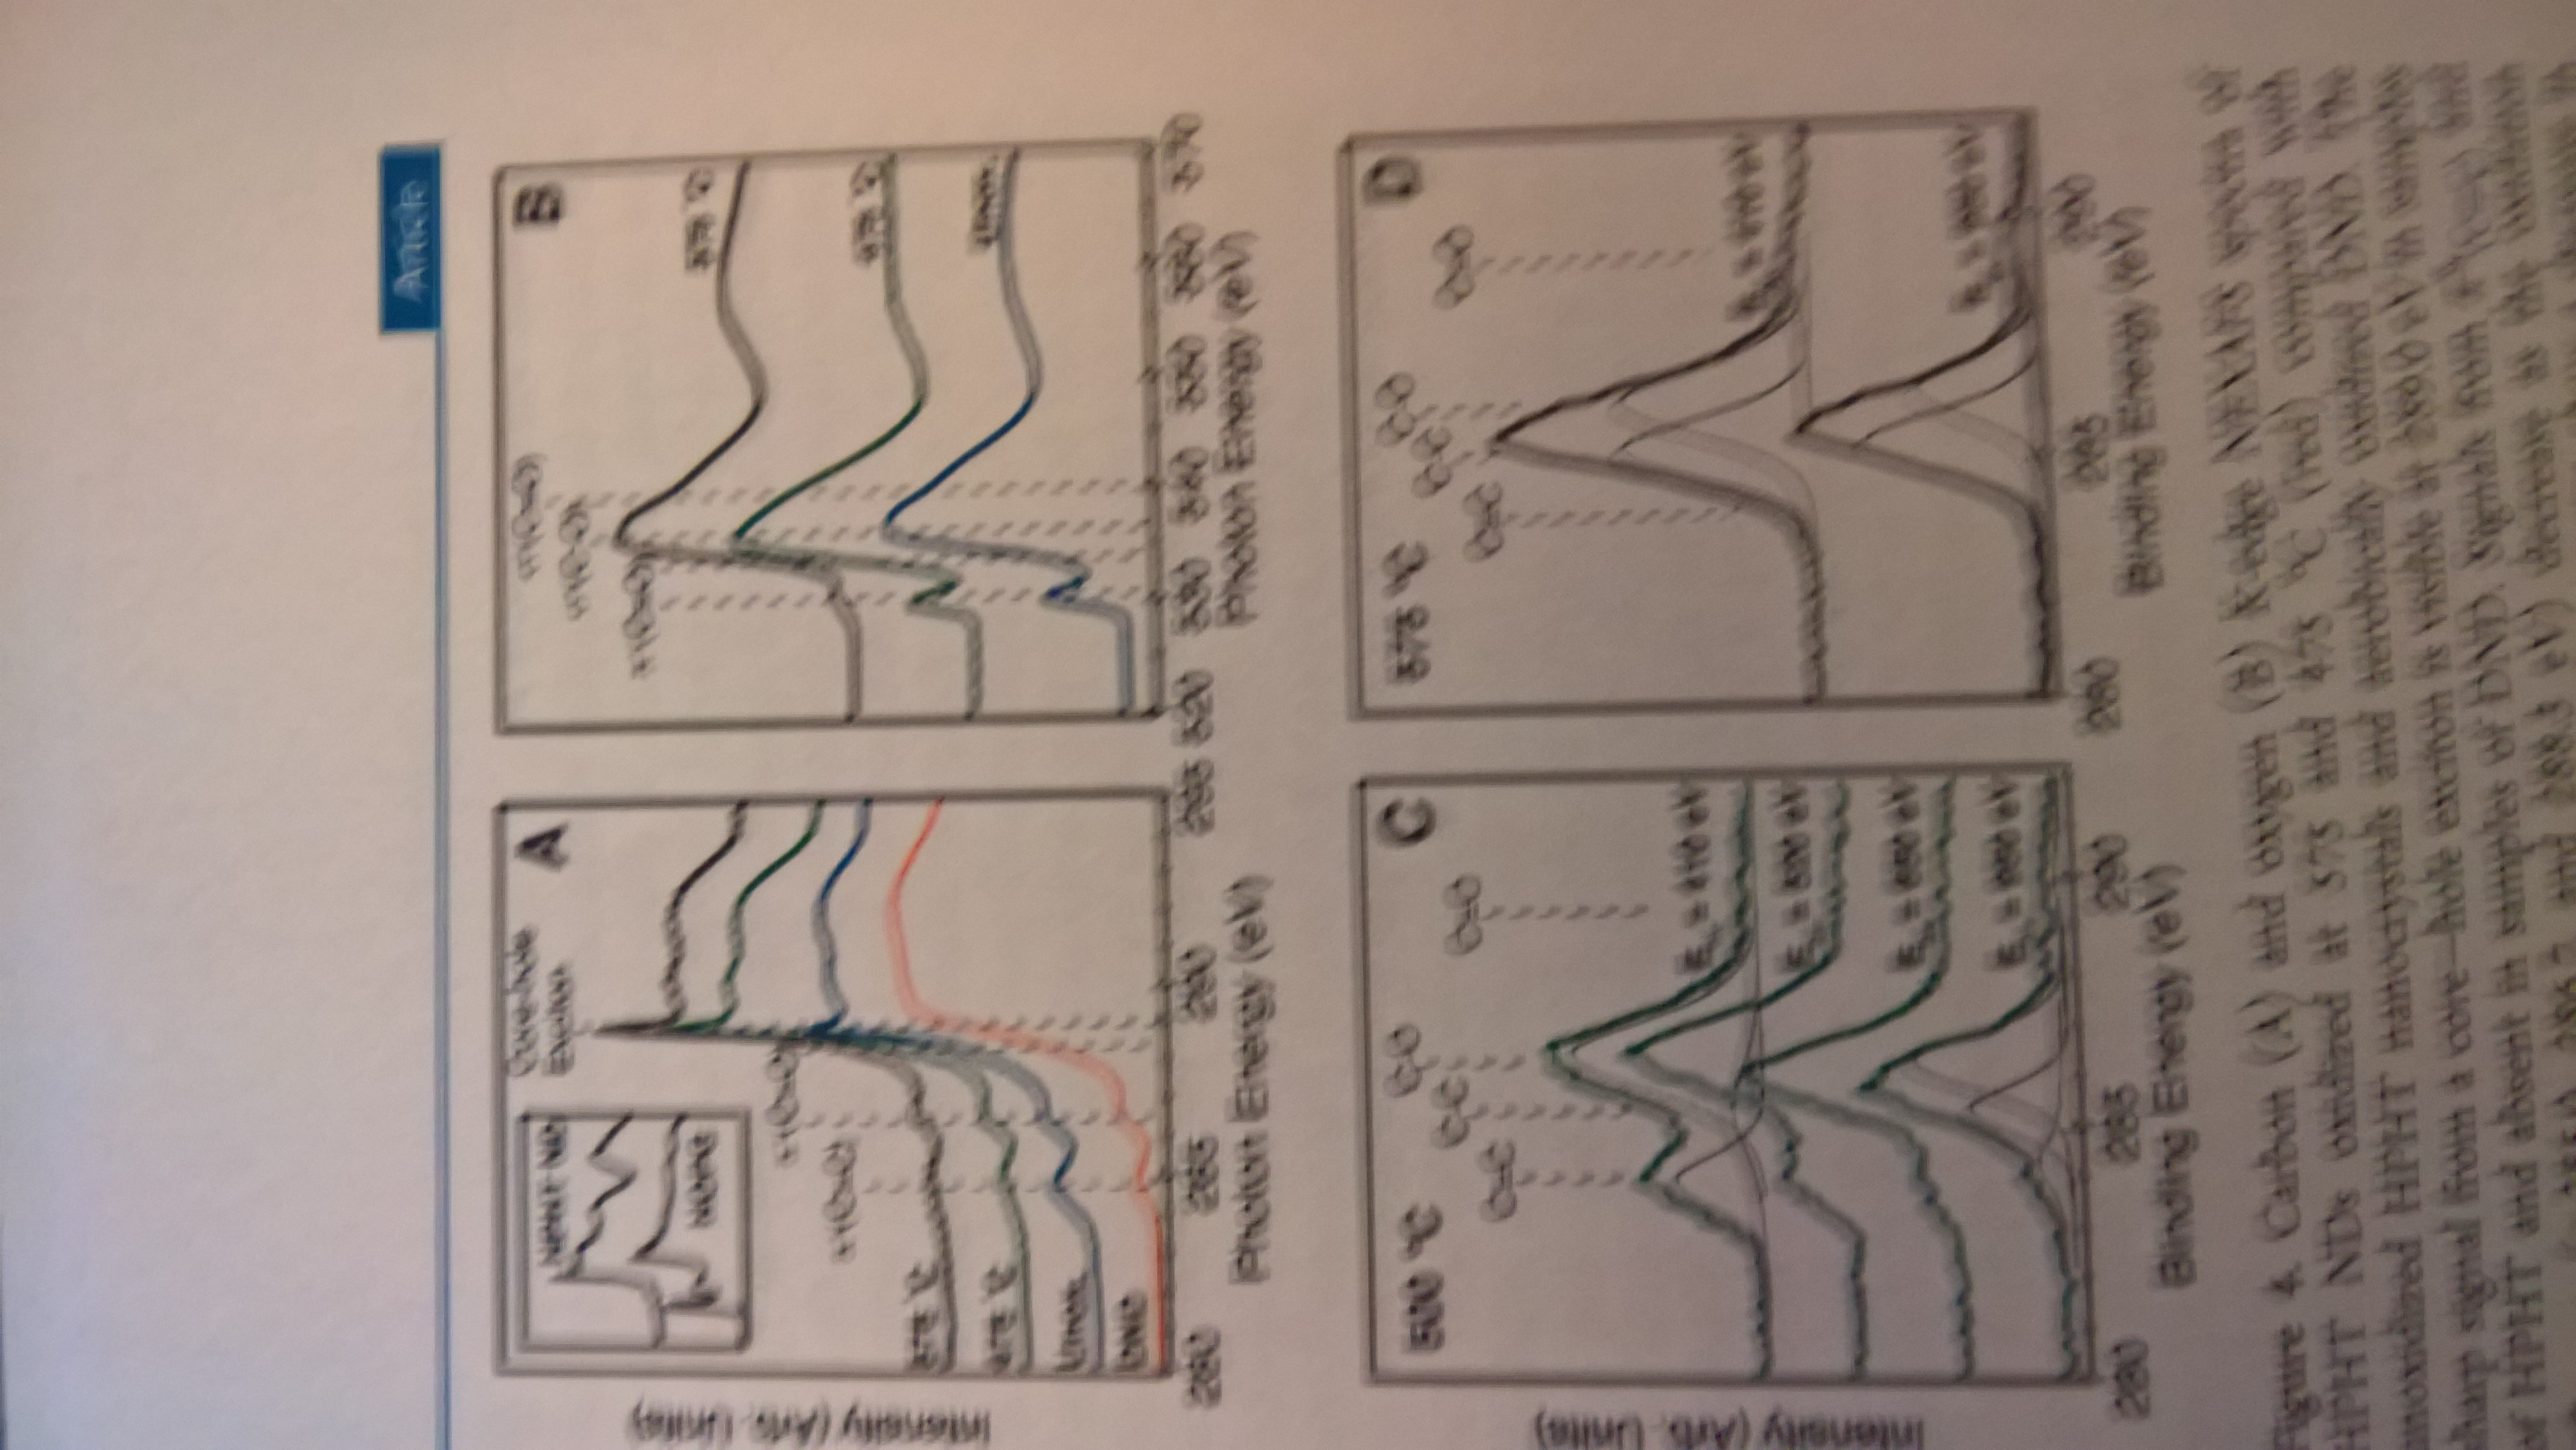
\includegraphics[width=0.7\linewidth]{../pic/WP_20160921_20_42_21_Pro_LI}
\caption{}
\label{fig:wp20160921204221proli}
\end{figure}

\paragraph{Before Oxidation} optical image after spincoating, excitation polarisation: confocal image, histogram of the distribution of peaks. SEM image.
\begin{figure}[h]
	\centering
	\includegraphics[height=0.7\linewidth]{../pic/WP_20160921_21_04_59_Moment}
	\caption{}
	\label{fig:wp20160921210459moment}
\end{figure}

\paragraph{After Oxidation} Confocal image of bright back ground. Gr1 center everywhere. Can't see pois.
\begin{figure}[h]
\centering
\includegraphics[height=0.7\linewidth]{../pic/WP_20160921_21_05_04_Moment}
\caption{}
\label{fig:wp20160921210504moment}
\end{figure}

\paragraph{Analysis} 
Comparasion if possible: different behaviour pre treatment between two batches
Possible reason: losing NDs due to Helium flow while cooling, GR1 getting closer to the surface due to oxidation caused size/thickness reduction.

%----------------------------------------------------------------------------------------
%	SECTION 4
%----------------------------------------------------------------------------------------

\section[H termination]{H termination}
\paragraph{Effect of H termination}
\begin{figure}[h]
\centering
\includegraphics[width=0.7\linewidth]{../pic/WP_20160921_21_05_16_Pro_LI}
\caption{}
\label{fig:wp20160921210516proli}
\end{figure}

NEA, band structure of diamond. Reduction of surface.
\paragraph{method} Plasma treatment, setup, apparatus.

\paragraph{why no pre characterisation} Conditions for Plasma treatment.

\paragraph{After H termination} Confocal image, optical image, excitation polarisation, time resolved PL with different incident polarisation.
\begin{figure}[h]
\centering
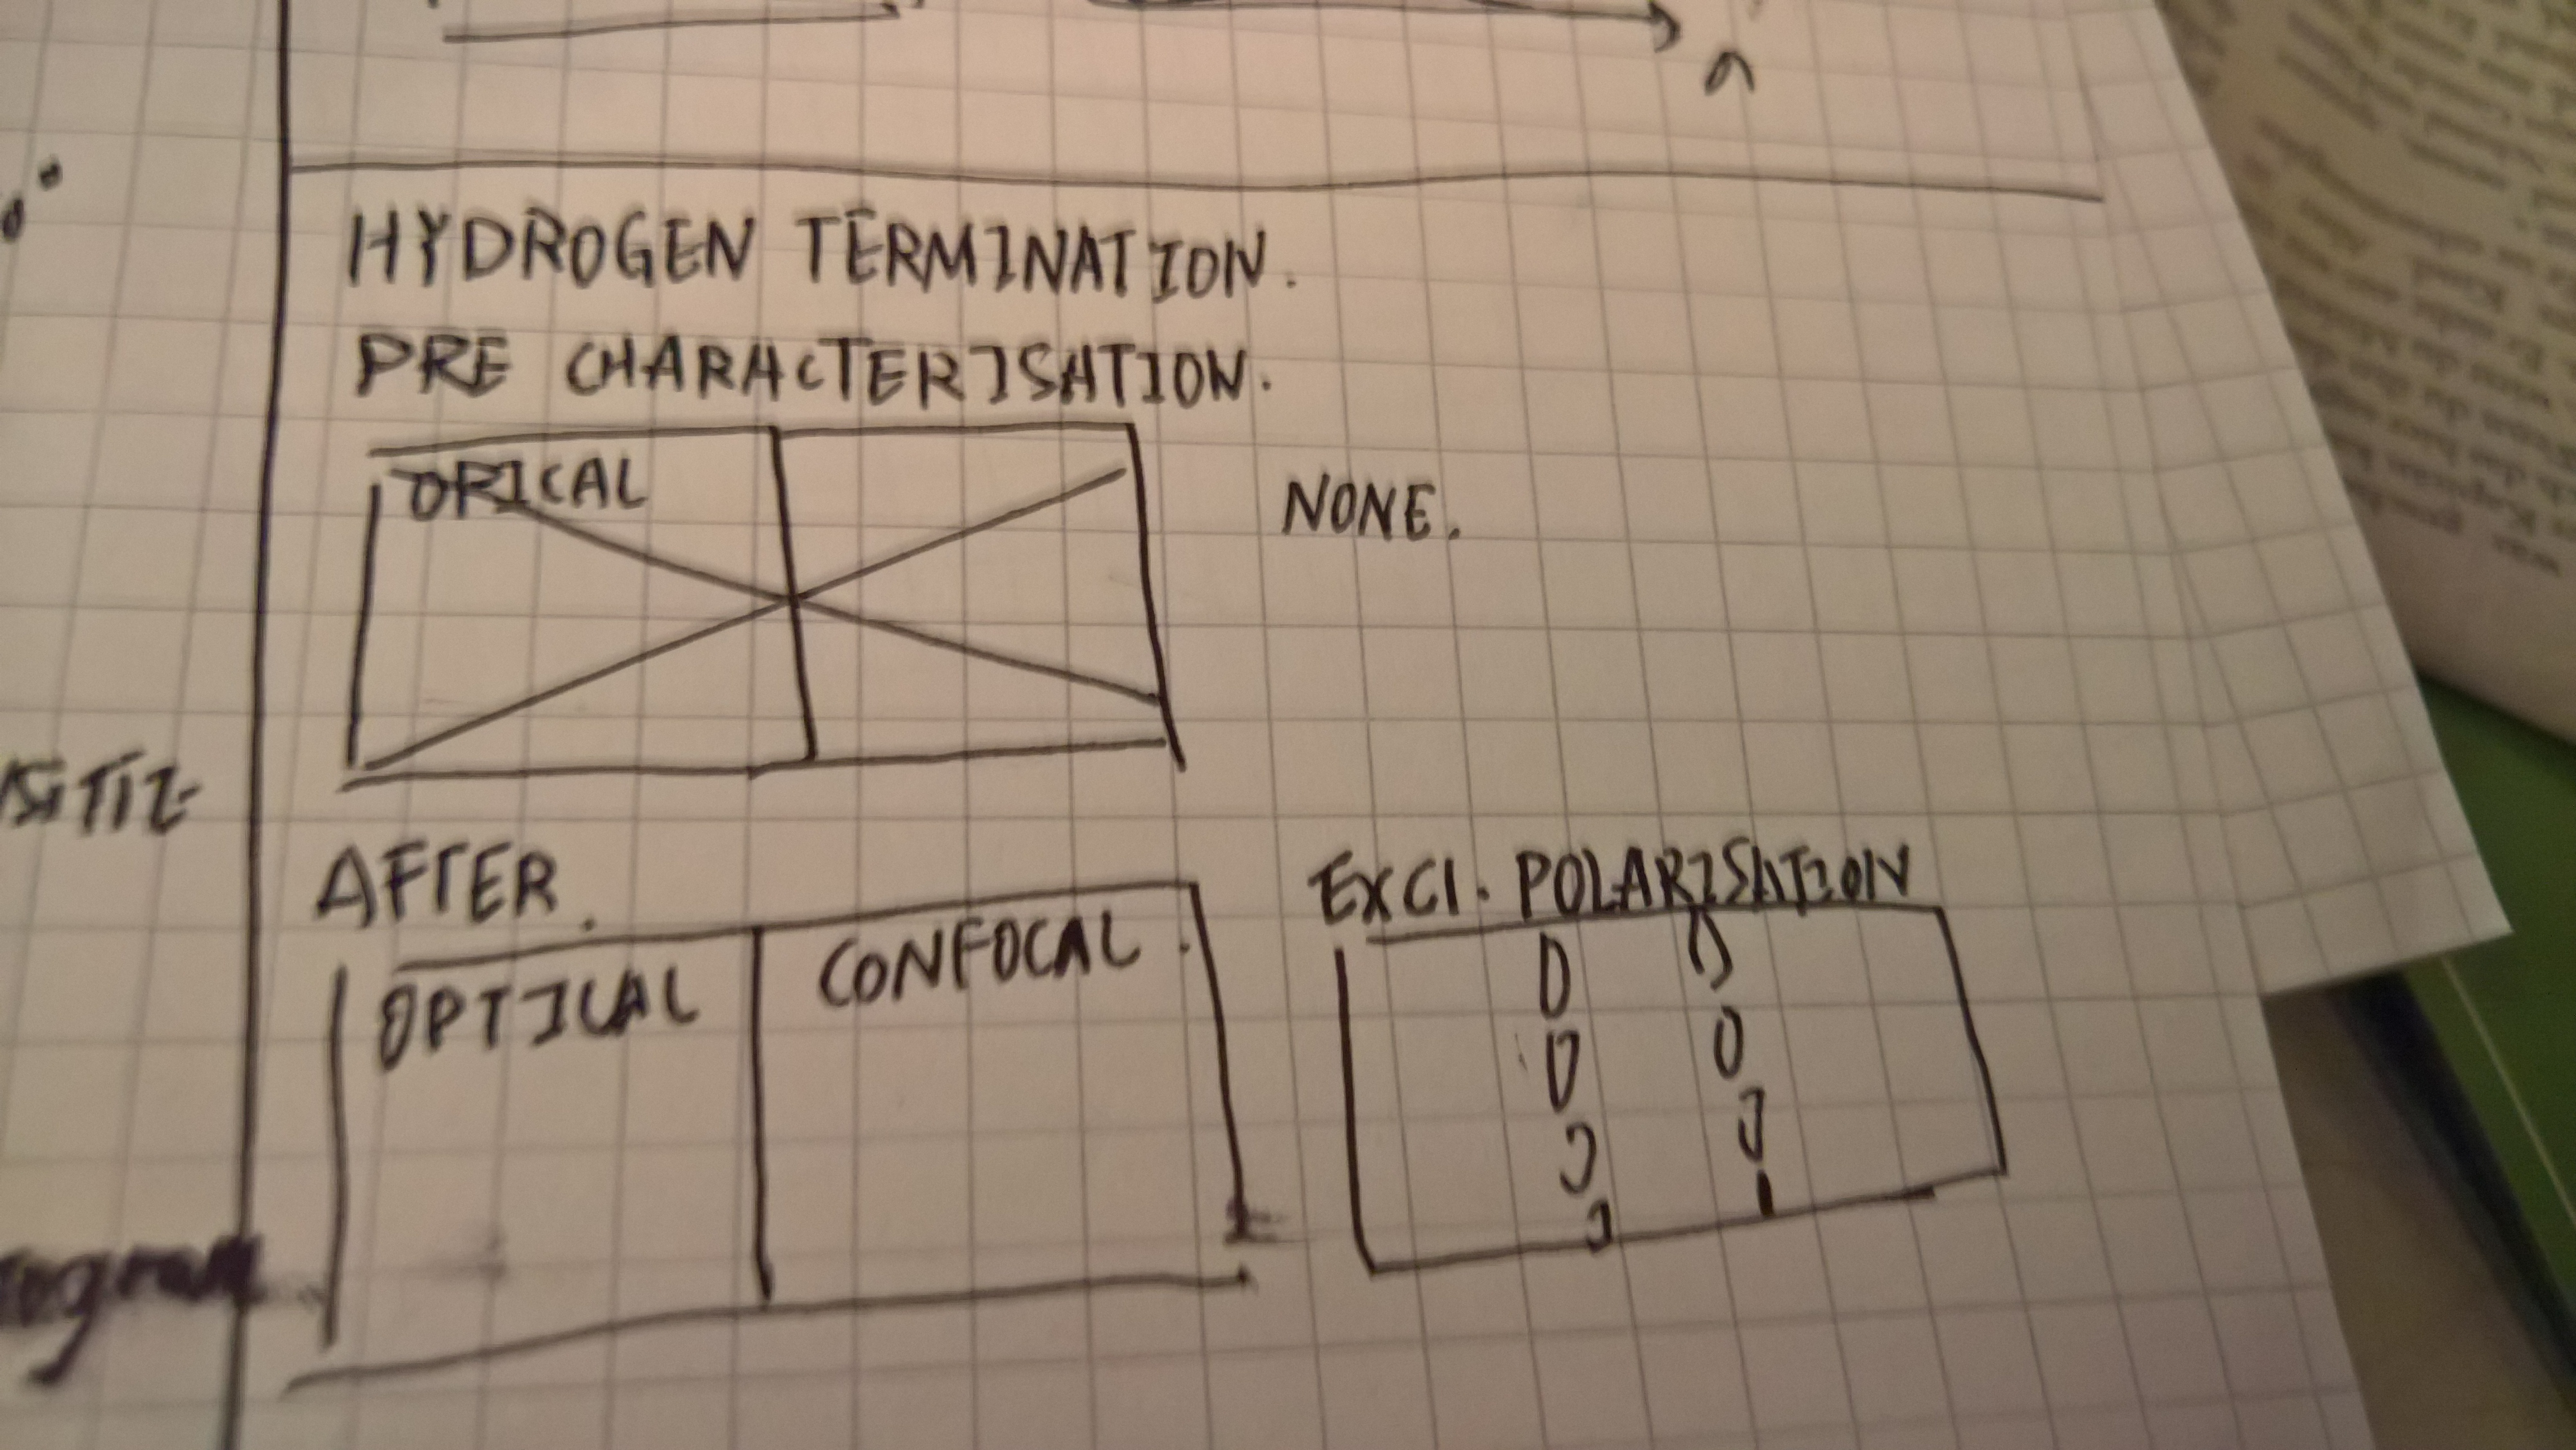
\includegraphics[width=0.7\linewidth]{../pic/WP_20160921_21_05_07_Pro_LI}
\caption{}
\label{fig:wp20160921210507proli}
\end{figure}
\begin{figure}[h]
\centering
\includegraphics[width=0.7\linewidth]{../pic/WP_20160921_21_05_13_Pro_LI}
\caption{}
\label{fig:wp20160921210513proli}
\end{figure}

\paragraph{Analysis} Within the instrumental limit of spectrometer, the spectral diffusion has been significantly suppressed. Possible reason.